\section{Signaturen der detektierten Teilchen}
Elektronische, myonische, tauonische und hadronische Zerfälle
des \Z-Bosons können aufgrund ihrer unterschiedlichen Signaturen in den
Detektoren identifiziert werden.
Die fünf Parameter, die im Versuch zur Charakterisierung eines Zerfalls verwendet werden, sind:
\begin{itemize}
  \item NCHARGED: Die Anzahl der geladenen Teilchen in den Spurdetektoren
  \item PCHARGED: Energie der Teilchen, berechnet aus den Messdaten der Spurdetektoren
  \item E\_ECAL: Energie, die im elektromagnetischen Kalorimeter deponiert wurde
  \item E\_HCAL: Energie, die im hadronischen Kalorimeter deponiert wurde
  \item COS\_THET: Polarwinkel des positiven Leptons bezüglich der Positronstrahlrichtung
\end{itemize}
Mit Beispielbildern der Auswertungssoftware \emph{GROPE} wird kurz beschrieben,
wie die vier Zerfallskanäle unterschieden werden können.
\subsection*{\Zee}
Beim \Zee-Zerfall werden zwei Spuren von Elektron und Positron in den Spurkammern detektiert.
Die Spuren enden im elektromagnetischen Kalorimeter,
in dem die gesamte Energie der beiden Teilchen deponiert wird (\autoref{img:sig:ee}).
Die Energiedeposition im hadronischen Kalorimeter ist minimal.
Durch Bhabha-Streuung treten viele Elektronen
mit einem kleinen Ablenkwinkel $\Theta$
von der Strahlrichtung auf.

\begin{figure}[H]
\begin{center}
  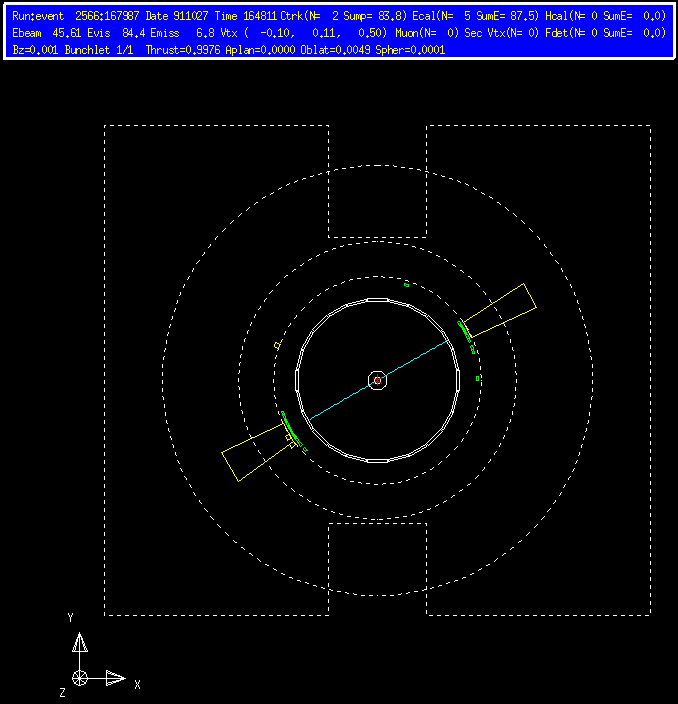
\includegraphics[width=0.6\textwidth]{../img/gropepics/ee1b.png}
  \caption{Signatur des Zerfalls \Zee: Elektron und Positron erzeugen zwei Spuren in den Driftkammern (blau)
  und deponieren anschließend ihre gesamte Energie im elektromagnetischen Kalorimeter (gelb).}
  \label{img:sig:ee}
\end{center}
\end{figure} 

\subsection*{\Zmm}
Auch Myon und Antimyon erzeugen zwei Spuren in den Spurdetektoren,
die Energie kann hier relativ genau bestimmt werden.
In den beiden Kalorimetern verlieren die Teilchen nur wenige GeV.
Sie werden schließlich in den Myonendetektoren registriert (\autoref{img:sig:mm}).

\begin{figure}[H]
\begin{center}
  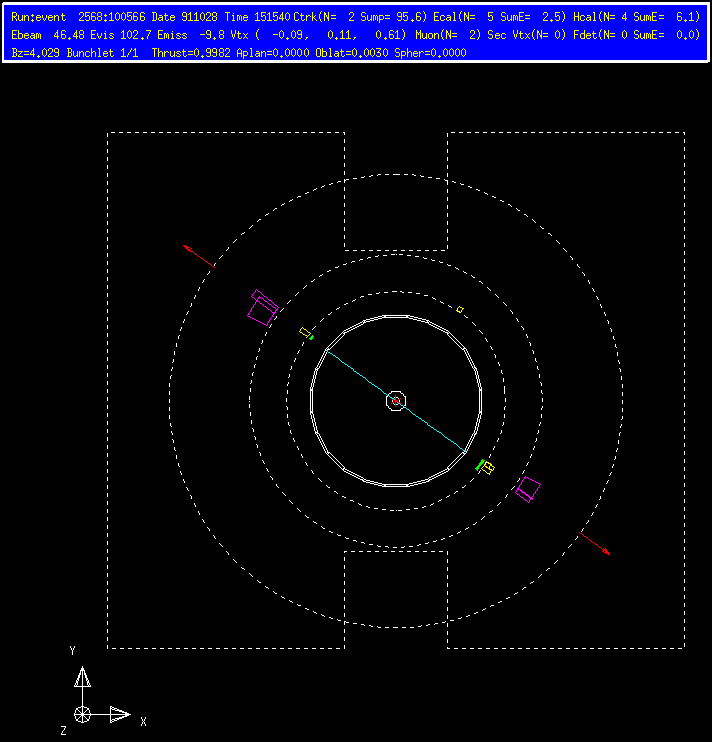
\includegraphics[width=0.6\textwidth]{../img/gropepics/mm1b.png}
  \caption{Signatur des Zerfalls \Zmm: Die beiden Teilchen werden im Spurdetektor erkannt (blau),
  deponieren wenig Energie in den beiden Kalorimetern (gelb und violett) und verursachen schließlich Ereignisse
  in den Myonendetektoren (rot).}
  \label{img:sig:mm}
\end{center}
\end{figure} 

\subsection*{\Ztt}
Da das \texttau-Lepton viele verschiedene Zerfallskanäle besitzt,
ist seine Signatur komplexer.
Meistens werden zwei Spuren detektiert,
es kommen aber auch Ereignisse mit vier oder sechs Spuren vor.
Sehr selten erfolgt die Detektion von drei oder fünf Spuren.
Die von dem Spurdetektor bestimmten Energien variieren über einen großen Bereich.
Ein größerer Teil der Energien wird im elektromagnetischen Kalorimeter abgegeben,
wenig im Hadronischen (\autoref{img:sig:tt}).

\begin{figure}[H]
\begin{center}
  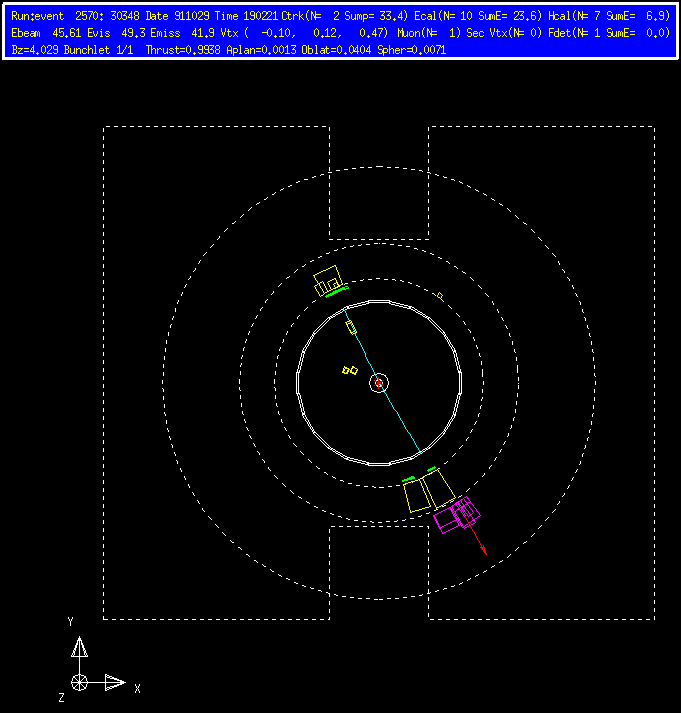
\includegraphics[width=0.6\textwidth]{../img/gropepics/tt1b.png}
  \caption{Signatur des Zerfalls \Ztt: In den Spurdetektoren werden zwei (oder auch mehr)
  Spuren detektiert (blau),
  ein Teil der Energie wird im elektromagnetischen Kalorimeter abgegeben (gelb) und wenig im Hadronischen (violett).}
  \label{img:sig:tt}
\end{center}
\end{figure} 

\subsection*{\Zqq}
Hadronische Zerfälle  besitzen eine charakteristische Signatur:
Die Zahl der Spuren ist sehr hoch, sie beträgt bis zu 35.
Die Energieabgabe erfolgt in beiden Kalorimetern (\autoref{img:sig:qq}).

\begin{figure}[H]
\begin{center}
  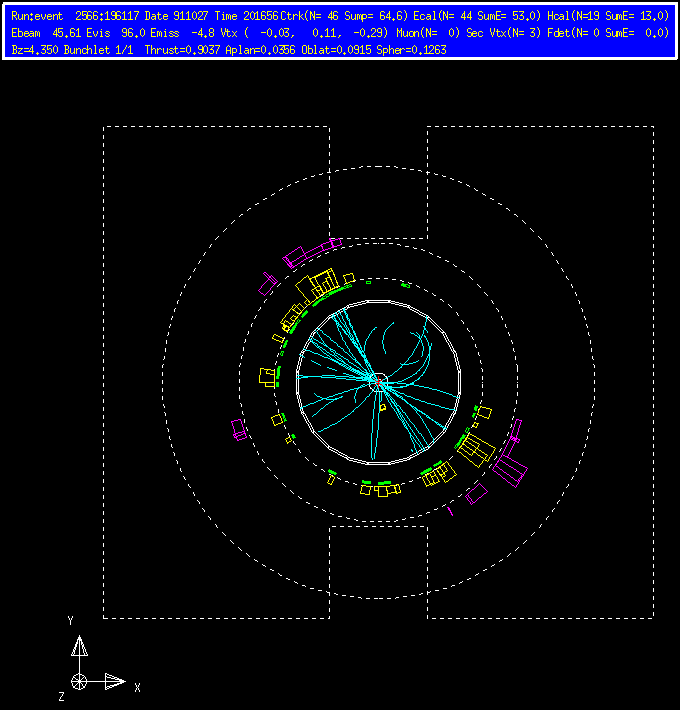
\includegraphics[width=0.6\textwidth]{../img/gropepics/qq1b.png}
  \caption{Signatur des Zerfalls \Zqq: Die Zahl der detektierten Spuren ist sehr hoch,
  Energieabgabe erfolgt in beiden Kalorimetern.}
  \label{img:sig:qq}
\end{center}
\end{figure} 